\section{Objectives} \label{chapter3:objectives}

% The objective of this thesis is to find a reconciliation of the two goals, by finding an equivalence between two approaches with different goals, in the case of streaming web applications.

The section \ref{chapter3:software-design} shows modularity is the best organization to improve maintainability of an application.
This organization is best supported by a functional approach.
Indeed, higher-order programming improves readability and maintainability.
However, higher-order programming, and modular programming in general, requires the use of a global memory store.

The section \ref{chapter3:software-efficiency} shows that to attain scalability, an application needs to be organized to distribute its memory store into independent silos to multiply the exclusive accesses.
Still, many works provide this global memory store interface to developers, because it is the best way to support the modularity advocated in section \ref{chapter3:software-design}.
This incompatibility between these two organization, and their goals is responsible for the shifts operated during the life of an application.
Huge developing efforts are made to translate manually from one organization into the other, and to maintain the implementation despites its unmaintainable nature.
% when the most pressing need shift from maintainability to performance, or vice versa.

In section \ref{chapter3:reconciliations}, we show different tentatives to reconciles the two organizations.
Most are satisfactory for specific domains, such as the high-performance computing.
It is profitable, as the expected speedup of developing an application with an adapted programming model compensates the huge development effort.
%  where it is accepted to spend long time developing an application to use thousands of accelerators to compute heavy calculation, because the expected speedup is profitable, compared to develop an application for all these thousands accelerators.
However, none are satisfactory in the case of web applications because the need for performance is always uncertain.
The development effort is not required at the beginning, hence its cost cannot be justified.
It is only when the audience increases, often with the revenue, that the cost for the development effort can be justified.
This situation illustrate the need for a programming model reconciling the two concerns, of maintainability and performance.
% Indeed, they all are too specific, and require too much from the developer to be accepted at a large scale.

% \comment{Here a table summarizing the different approaches, and the sweet spot.}

\begin{table}
\begin{tabular}{l|l|l|l}
             & Maintainability         & Performance           & Both\\\hline
General      & Functional Programming  & Message-passing       & Loop parallelization\\
Web          & Javascript              & Pipeline architecture & ø
\end{tabular}
\caption{Summary of the state of the art}
\label{tab:chapter3:objectives:summary}
\end{table}

Our objectives is to find an equivalence between these two organization, specifically for the case of web applications.
To do so, we focus on the Javascript programming language, and specifically, the node.js interpreter.
As explained in the end of chapter \ref{chapter2}, the execution model of Javascript is similar to a pipeline.
We intend to split a node.js application into a parallel pipeline of stages.

The contribution of this thesis is organized in two chapters, as illustrated in figure \ref{fig:chapter3:objectives:roadmap}.
In chapter \ref{chapter4} I present the extraction of a pipeline of operations from a Javascript application.
I show that such pipeline is similar to the one exposed by Promises, and I propose a simpler alternative to the latter called Dues.
However, these operations still require a global memory for coordination so they are not executed in parallel.
In chapter \ref{chapter5}, we present the isolation of the operations into isolated containers called Fluxions. 

\begin{figure}[h!]
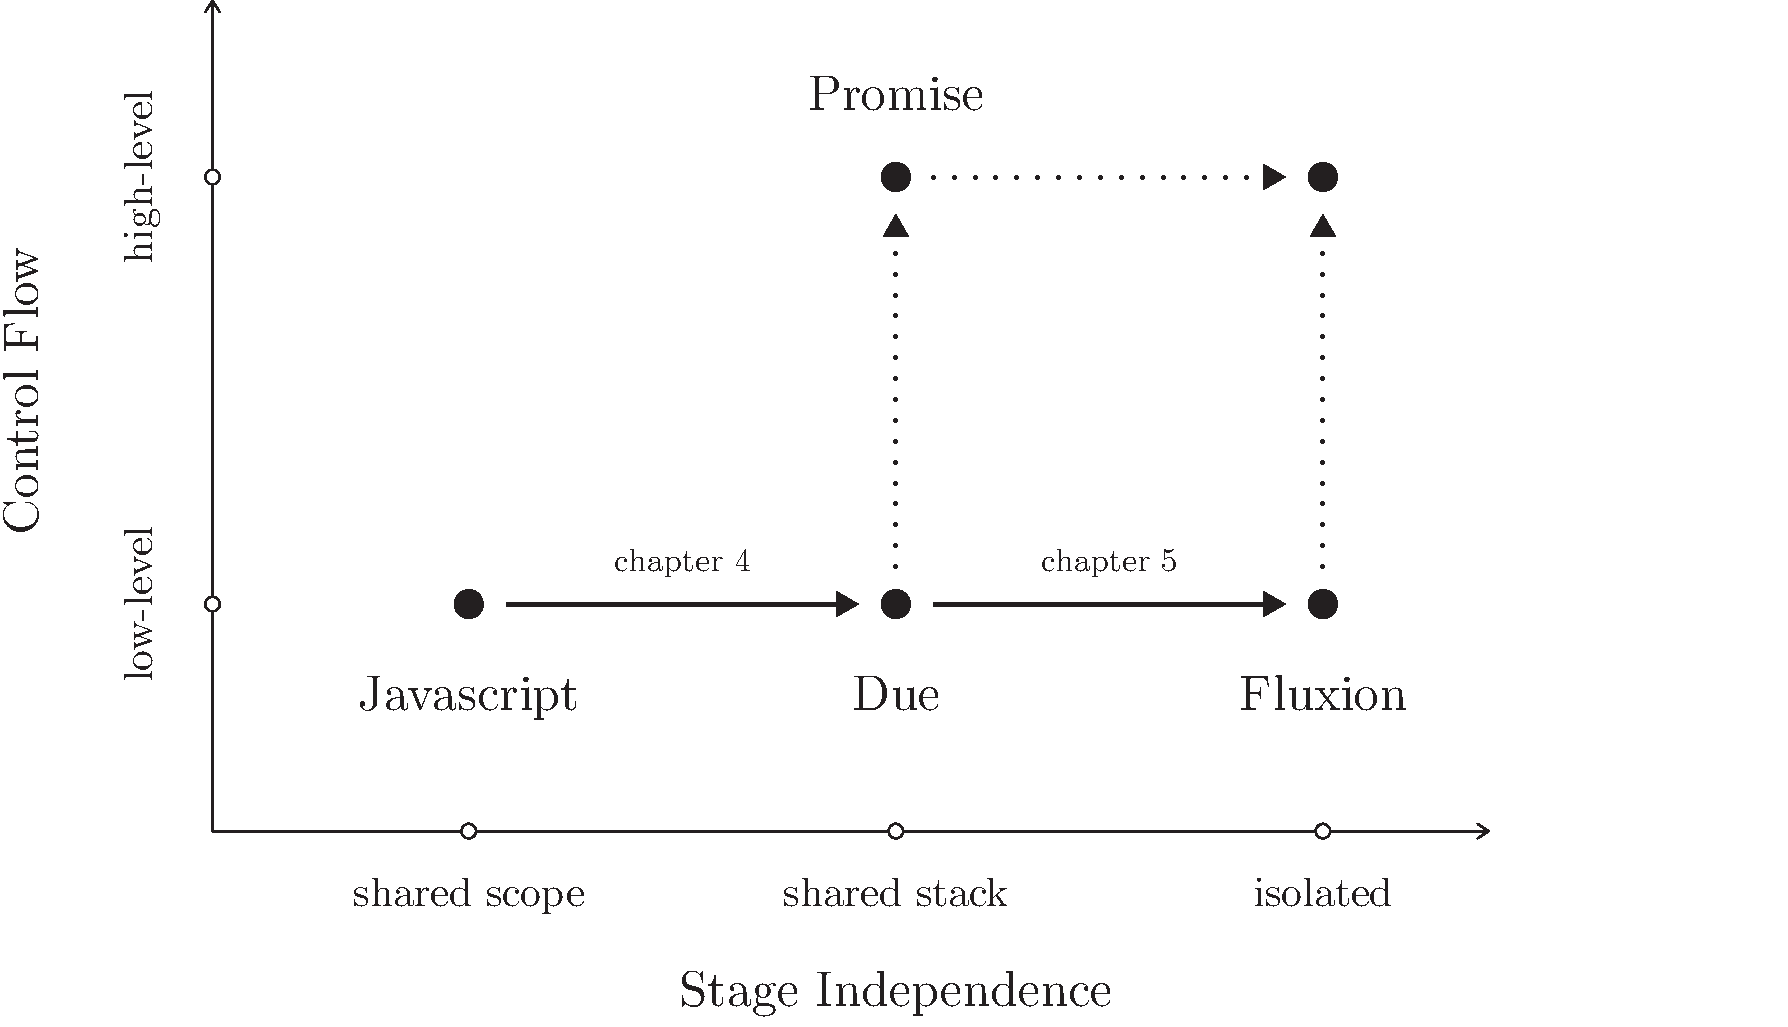
\includegraphics[width=1\textwidth]{../ressources/roadmap.pdf}
\caption{Roadmap for this work}
\label{fig:chapter3:objectives:roadmap}
\end{figure}

\endinput

We show that there is no languages that features higher-order functions to improve modularity, a common memory store easy to develop with, but at the same time provides scalable concurrency.

We aim at filling this gap, and for a concrete example, focus our work on the Javascript programing language.
Indeed, Javascript features higher-order functions, is highly-used in concurrent context, but lacks scalable concurrency.

Our work is divided into two contributions: Due and Fluxions.

-> Schema roadmap.